\chapter{Hardware Design}

\section{Original Leg Design}

\subsection{Leg Hip}
The original leg 'hip' was designed by Ben Bingham in 2016 in completion of his undergraduate vacation work as seen in \cref{fig:original-hip}.

The 'hip' was constructed of 6 mm perspex sheet in a box design with metal L connectors to join the sheets securely. The design of the 'hip' allowed the motor drivers as well as the microcontroller to be mounted on one leg, with space provided for an extra leg for future two-legged movement. 

\begin{figure}
\centering
\includegraphics[clip, trim =0cm 0cm 0cm 0cm, page =1, width=0.4\textwidth]{images/mechanical/hip-6mm-360x360}
\caption{Original 'hip' design by Ben Bingham, 2016.}
\label{fig:original-hip}
\end{figure}

\subsection{Leg Guide}
The guiding system consisted of two parallel steel rods with ball bearings mounted on the 'hip'. 

\subsection{Problems with Design}

The leg mounting plate went through three design iterations after the original 'hip' design before the final design was created, as seen in \cref{fig:CAD mounting plate final design}.

The original 'hip' design had the following mechanical design flaws:

\begin{enumerate}
\item The 6 mm perspex box construction with on-board microncontroller and motor drivers is too heavy for efficient jumping action when compared to similar designs like \cite{Duperret} (1.3 kg), \cite{Kalouche2016} (2.5 kg), \cite{Wang2012} (4.2 kg) where there is a high leg torque to mass ratio.
\item The ball bearings are particularly heavy.
\item The mounting of the leg guide places a significant torque in all three cartesian coordinates being off-center from the center of mass.
\item The design of the leg guide requires the two steel rods to be perfectly parallel to remove resistance to movement, which is difficult to achieve practically.
\end{enumerate}

These problems were accounted for by replacing the original 'hip' with a rigid aluminium mounting plate with off-board microcontroller and motor drivers. The leg guide consisting of parallel steel rods and ball bearings was replaced with a linear guide as seen in \cref{fig:drylin-linear-guide}.  

\begin{figure}
\centering
\includegraphics[width=0.8\textwidth]{images/mechanical/leg-mount-annotated} 
\caption{Final leg design mounted to platform and linear guide: front.}
\label{fig:Final leg design - front}
\end{figure}

\begin{figure}
\centering
\includegraphics[width=0.8\textwidth]{images/mechanical/encoder-mount-annotated} 
\caption{Final leg design mounted to platform and linear guide: back.}
\label{fig:Final leg design - back}
\end{figure}

\section{Mechanics and Construction}

\subsection{Alumnium Mounting Plate Design}

\begin{figure}
\centering
\subfloat[][CAD mounting plate V1.]{
\includegraphics[clip, trim=2cm 0cm 16cm 1cm, page = 1, width=0.3\textwidth]{images/mechanical/laser-test-print-V1} 
\label{fig:CAD mounting plate V1}
}
\subfloat[][CAD mounting plate V3.1.3.]{
\includegraphics[clip, trim=5cm 10cm 14cm 2cm, page = 1, width=0.3\textwidth]{images/mechanical/laser-test-print-V313} 
\label{fig:CAD mounting plate V3.1.3}
}

\subfloat[][CAD mounting plate final design.]{
\includegraphics[clip, trim=0cm 21cm 9cm 0cm, page = 1, width=0.6\textwidth]{images/mechanical/main-plate-final} 
\label{fig:CAD mounting plate final design}
}
\caption{Leg mounting plate iterations.}
\label{fig:Leg mounting plate iterations}
\end{figure}

\begin{figure}
\centering
\includegraphics[width=0.6\textwidth]{images/mechanical/driver-mount-plate.pdf} 
\caption{Motor driver interface mounting plate.}
\label{fig:Motor driver interface mounting plate}
\end{figure}

\subsection{Leg Linkage and Foot Design}

The 4-bar linkage design of the leg was originally constructed by Ben Bingham in 2016 for completion of his undergraduate engineering vacation work in the mechatronics lab. The leg was constructed as follows:

\begin{itemize}
\item Three sets of rotational joints make up the linkage system. The joints were 3D printed using ABS plastic and used 3 mm screws to connect to the aluminium leg sections.
\item 8 mm loctite nut, bolt and washer combinations connected the joint components with perspex discs to reduce friction between the joints.
\item The aluminium leg sections were constructed of 25 mm diameter tubing to form a leg of 0.15 m and 0.3 m sections including the joints. 
\end{itemize}

\begin{figure}
\centering
\includegraphics[width=0.6\textwidth]{images/experiments/lateral-slipping} 
\caption{Leg foot lateral slipping.}
\label{fig:foot-slipping}
\end{figure}







\subsection{Testing Platform}


\begin{figure}
\centering
\includegraphics[width=0.8\textwidth]{images/mechanical/drylin-linear-guide.png} 
\caption{igus DryLin T - Low-profile linear guide.}
\label{fig:drylin-linear-guide}
\end{figure}


\begin{figure}
\centering
\includegraphics[width=0.8\textwidth]{images/mechanical/back-shot.png} 
\caption{Linear guide mounted leg model (CAD Solidworks assembly).}
\label{fig:Linear guide mounted leg model}
\end{figure}


\section{Mass Distribution}



Servo drive mounting card = 50.7g
Servo drive = 123.9g
T-Motor U10 Plus = 500g

Savings = 349.2g

Complete leg = 2.2kg
Leg = 0.5kg
Plate = 0.7kg
Motors = 1kg

The center of mass (COM) moves negligibly with the foot position. To calculate a COM for placement of the linear guide mount and iNemo, a intermediate radial foot position of $0.25 m$ was chosen - this position set-point was used for compliant landing and launch sequences. ...

% Please add the following required packages to your document preamble:
% \usepackage[table,xcdraw]{xcolor}
% If you use beamer only pass "xcolor=table" option, i.e. \documentclass[xcolor=table]{beamer}
\begin{table}[]
\centering
\begin{tabular}{llll}
\textbf{Colour legend}                          & \textbf{Component}    & \textbf{No.} & \textbf{Mass (g)} \\
\cellcolor[HTML]{FE0000}                        & T-Motor U10 Plus      & 2            & 424.56            \\
\cellcolor[HTML]{CB0000}                        & Mounting Plate        & 1            & 378.86            \\
\cellcolor[HTML]{010066}{\color[HTML]{000000} } & Linear Guide Carriage & 1            & 100.37            \\
\cellcolor[HTML]{3531FF}                        & ABS Motor Joint       & 2            & 50.55             \\
\cellcolor[HTML]{3531FF}                        & Long Linkage          & 2            & 46.40             \\
\cellcolor[HTML]{3531FF}                        & Joint                 & 5            & 39.83             \\
\cellcolor[HTML]{3531FF}                        & Foot Joint            & 1            & 39.63             \\
\cellcolor[HTML]{3531FF}                        & Short Linkage         & 2            & 12.81             \\
\cellcolor[HTML]{3531FF}                        & Washer Bearing        & 3            & 2.41              \\
\textbf{Total:}                                 & \textbf{}             & \textbf{}    & \textbf{1793.88} 
\end{tabular}
\caption{Solidworks leg assembly mass distribution.}
\label{my-label}
\end{table}

\begin{figure}
\centering
\subfloat[][Mass distribution graphic.]{
\includegraphics[clip, trim=5cm 2cm 4cm 2cm, page = 1, width=0.7\textwidth]{images/mechanical/assembly-com-distribution.pdf} 
}
%\subfloat[][Mass distribution colour legend (grams).]{
%\includegraphics[width=0.3\textwidth]{images/mechanical/com-distribution} 
%}

\subfloat[][Center of mass of leg assembly.]{
\includegraphics[clip, trim=5cm 2cm 5cm 5cm, page = 1, width=1\textwidth]{images/mechanical/assembly-com.pdf} 
}
\caption{Mass distribution of leg assembly.}
\label{fig:Mass distribution of leg assembly.}
\end{figure}

...

\section{Electronics and Communication}
\subsection{Accelerometer and Gyroscope}
\subsection{Distance Sensor}
A distance sensor was mounted to the base of the mounting plate, as seen in \cref{fig:Final leg design - back}. This provided feedback of the height of the leg's center of mass above the ground.

The leg height was used for height control as well as flight phase determination.

An infra-red distance sensor was chosen with a narrow beam width - this ensures there is minimal reflection off surrounding objects that could interfere with distance readings. The beam reflects off the surface of the ground and a time-of-flight calculation is used to determine distance. Infra-red is open to possible interference from surrounding fluorescent light sources, and this can be accounted for by using it in an area out of direct line of site of light sources. Infra-red was chosen because it is cheaper than an equivalent laser distance sensor.

The Pololu Carrier with Sharp GP2Y0A60SZLF Analog Distance Sensor was used. It requires a $3\ V$ voltage source which can be supplied directly from the micrcontroller which runs off the same voltage. 

The distance sensor outputs an analog signal which is related to the height. This analog signal is fed into the ADC of the microcontroller and using a linear relationship is mapped to the distance. 

The Pololu distance sensor has a range of $10-150\ cm$, which is more than enough for the intended hopping height of $20-50\ cm$ due to the testing rig limits.

The height sensor was calibrated by setting it at $0.1\ m$ from a surface and using a scaling factor to adjust the linear relation between distance and voltage until an accurate value was achieved. 

A 3D printed carrier was designed for the distance sensor which offset the sensor from the mounting plate and placed it in a central location above the linear guide.

\subsection{Microcontroller}
The microcontroller had to meet the following specifications:
\begin{itemize}
\item 4 x UART Ports
\item 1 x ADC
\item 1 x Floating point unit
\item DMA Capabilities
\item USB Debugging
\item 5V tolerant UART ports
\end{itemize}

Being familiar with the STM32 series of microcontrollers, a STM32F4 board was chosen and met the above specifications with two additional USART ports for future peripheral needs.

\section{Motors and Drivers}

\subsection{Driver Selection}

\begin{figure}
\centering
\subfloat[][AMC DigiFlex Performance Servo Drive.]{
\includegraphics[width=0.5\textwidth]{images/driver/driver.jpg} 
}
\subfloat[][AMC DigiFlex Performance Servo Drive mounting card.]{
\includegraphics[width=0.5\textwidth]{images/driver/mounting-card.jpg}
} 
\caption{AMC Servo Drive and Mounting Card.}
\label{fig:AMC Servo Drive and Mounting Card}
\end{figure}

\subsection{Motor Selection}

In the study by \cite{Kalouche2016} various COTS (commercial off the shelf) motors were compared using the thermal specific torque as a performance measure. The T-Motor U10 Plus was found to have the highest thermal specific torque at $0.42 \frac{Nm}{kgC^o } \text{ at } r_{gap} = 40 mm$ \cite{Kalouche2016}. When compared to the custom made MIT Cheetah motors at $0.71 \frac{Nm}{kgC^o } \text{ at } r_{gap} = 49 mm$ found in \cite{Wang2012} they perform favourably. 

\begin{figure}
\centering
\includegraphics[clip, trim=0cm 5cm 0cm 2cm, width=0.4\textwidth]{images/motor/TMotorU10Plus} 
\caption{T-Motor U10 Plus Brushless DC Motor.}
\label{fig:TMotorU10Plus}
\end{figure}

\subsection{Motor Model Calculations}

\subsubsection{Experimental Calculation of $K_t$ and $K_e$}
The motor torque constant, $K_t$, was calculated using the torque current relation $\tau = K_tI$. The leg was modelled as a virtual spring-damper system, as seen in \cref{fig:Leg spring-damper virtual model}. 

The spring constant, $K_{s1}$, was set to $200\ [N/m]$, and the damping and torsional spring-damping constants were set to zero. $K_t$ was tuned until the theoretical foot force matched the practical foot force measured via a scale. The leg was fixed at a set height imposing a radial offset on the virtual spring-damper system.

For a spring constant of $200\ [N/m]$ and a radial offset of $0.15\ m$ a theoretical foot force of $K_{s1}\Delta r = 30\ N$ was expected. A mass of approximately $3\ kg$ was measured with $K_t = 0.08\ [Nm/A]$ set in the virtual leg model controller, resulting in a foot force of $3\ kg \times 9.81\ m/s^2 = 29.43\ [N]$. 

The study in \cite{Kalouche2016}, using the same T-Motor U10 Plus motors, calculated a torque constant of $K_t =  0.072\ [Nm/A]$. This confirms the experimental results obtained above.

For an ideal motor at a constant operating point, $K_e$ will equal $K_t$, as shown in \cref{eqn:ktke}.

\begin{equation} \label{eqn:ktke}
\begin{aligned}
&V_t = K_e\omega_m + IR_m \\
&\tau_m = K_t I \\
&P_{elec.} = V_t I = K_e \omega_m I + I^2 R \\ 
&P_{mech.} = \tau_m \omega_m = K_t I \omega_m \\
&P_{loss.} = I^2 R_m \\
&P_{elec.} = P_{mech.} + P_{loss.} \\
&\therefore K_e\ [V/rad/s]= K_t\ [Nm/A] = 0.08
\end{aligned} 
\end{equation}

\subsubsection{Calculation of $R_m$ and $L_m$}
The resistance and inductance of the 3 phase windings of the motor were calculated using a lab multimeter to be $R_m = 47.5\ m\Omega$ and $L_m = 35\ \mu H$ respectively. 

Brushless DC motor windings are usually connected in WYE formation, as seen in \cref{bldc-wye-connection}. This means the measured values for resistance and inductance were line-to-line values and had to be divided by two to get the per phase values above.

\begin{figure}
\centering
\includegraphics[width=0.4\textwidth]{images/motor/wye.jpg} 
\caption{WYE connected BLDC motor windings.}
\label{fig:bldc-wye-connection}
\end{figure}

\subsubsection{Calculation of $J_m$}
In order to calculate the moment of inertia of the motor, $J_m$, the ratio of acceleration torque to acceleration to steady state needs to be found. By commanding a DC equivalent current input of $1\ A$ and measuring the time taken to reach a steady state velocity, \cref{eqn:Jm} can be used to calculate $J_m$. The velocity vs. time plot used can be seen in \cref{fig:jm-plots}.

\begin{equation} \label{eqn:Jm}
\begin{aligned}
J_m &= \frac{T_{acc.}[N/m]}{a[m/s^2]} \\
&= \frac{IK_t}{a} \\
&= \frac{IK_t}{\frac{\Delta v}{\Delta t}}\ [kg/m^2]
\end{aligned}
\end{equation}

where $I=1\ A$, $K_t=0.08\ Nm/A$, $\Delta v = 1313.906\times \frac{2\pi}{60}\ rad/s$ and $\Delta t = 588.889\times10^{-3}\ s$.

This results in a motor moment of inertia of $J_m = 3.424 \times 10^{-4}\ [kg/m^2]$.

\subsubsection{Calculation of $B_m$}

The motor damping or viscous friction, $B_m$, was assumed to be negligible. Brushless DC motors have near zero damping and will have little effect on the simulated motor model.

\begin{figure}
\centering
\includegraphics[width=0.5\textwidth]{images/driveware/current-velocity-response} 
\caption{Velocity vs. time plot for 1A equivalent DC command.\\
(500 rpm; 500 ms/div)}
\label{fig:jm-plots}
\end{figure}

\subsubsection{Calculation of $\tau_e$ and $\tau_m$}
The electrical and mechanical time constants of the motor, $\tau_e$ and $\tau_m$ respectively, can be used to plot a root-locus plot with poles at $-\tau_e$ and $-\tau_m$ as can be seen in \cref{...}. This is useful when designing a current controller for the system. $\tau_e$ and $\tau_m$ can be calculated using \cref{eqn:motor-time-constants}.

\begin{equation} \label{eqn:motor-time-constants}
\begin{aligned}
&K_m = \frac{1}{B_m} \\
&\tau_m = \frac{J_m}{B_m} \\
&K_e = \frac{1}{R_m} \\
&\tau_e = \frac{L_m}{R_m} 
\end{aligned}
\end{equation}

From \cref{eqn:motor-time-constants} and using the previously calculated motor constants, $\tau_e = 7.368 \times 10^{-4}$ and $\tau_m = 3.424 \times 10^{-4}$. This is assuming the motor viscous friction $B_m$ is insignificant which is usually the case in mechanically well made BLDC motors.

The resulting motor model open loop root-locus plot can be seen in \cref{fig:ol-motor-rlocus}. As expected the system has only negative real roots and will be stable in open loop.

\begin{figure}
\centering
\includegraphics[width=1\textwidth]{images/motor/ol-motor-rlocus} 
\caption{Motor model open loop root-locus plot.}
\label{fig:ol-motor-rlocus}
\end{figure}


\subsection{Driver Configuration}

The AMC drivers allow extensive customisation. After the motor, encoder, and general communication control parameters are configured, the PID control loops of the drivers can be configured, as seen in \cref{fig:AMCControlLoops}.

The motor drivers were initially configured with both on-board PID current and position control loops enabled. This allowed initial modelling of the motors, configuring of the motor encoders, and determining of the position limits (in counts). For control of the leg, the position control loop was finally implemented on the STM32F4 microcontroller, while using the existing current control loop of the motor drivers.

The AMC drivers were configured using the AMC Driveware configuration software, which provided an oscilloscope to measure the relevant motor responses as seen in \cref{fig:jm-plots,,fig:current-tuning-plots,,fig:position-tuning-plots}.

\begin{figure}
\centering
\includegraphics[clip, trim=2cm 5cm 2cm 8cm, page = 114, width=1\textwidth]{pdfs/AMC_DriveWareSoftwareManual.pdf} 
\caption{AMC DigiFlex Performance Servo Drive control loops (AMC, 2014).}
\label{fig:AMCControlLoops}
\end{figure}

\subsubsection{Current Control Loop}

By using a 1 A 120Hz square wave current command the current PI control loop was tuned, as seen in \cref{fig:current-tuning-plots}. Initially both  the proportional gain, $K_p$, and the integral gain, $K_i$, were set to zero. $K_p$ was slowly increased until the final amplitude of the current output just started to overshoot. $K_i$ was then set to minimize the steady state error. 

Values of $K_p = 0.277$ and $K_i = 0.262$ were obtained. Both motors were found to operate optimally with the same PI gain values.

\begin{figure}
\centering
\subfloat[][Motor driver current loop pre-tuning.\\ 
(200 mA; 5 ms/div)]{
\includegraphics[width=0.5\textwidth]{images/driveware/current-pre-tuning-plot.png} 
}
\subfloat[][Motor driver current loop tuning - 1A 120Hz square wave command.\\(1 A; 1 ms/div)]{
\includegraphics[width=0.5\textwidth]{images/driveware/current-tuning-plot.png} 
}
\caption{Motor driver current loop tuning plots.}
\label{fig:current-tuning-plots}
\end{figure}

\subsubsection{Position Control Loop}
The on-board AMC motor driver control loop was set up to test the encoder configuration. The encoder and relevant position limits can be seen in \cref{sec:motor-encoders}. 

A 1Hz sinusoid was used to tune the PID control loop gains. Values of $K_p = 0.0005793$, $K_i = 0.0006052$ and $K_d = 2.769e-9$ were found to achieve optimal set-point tracking as seen in \cref{fig:position-tuning-plots}. The sinusoidal set-point can be seen in white and the position feedback in yellow. A 10-30 ms lag time can be seen due to the inertial load. This lag time causes a dead-band which should be considered when implementing a controller. 

These tests were performed with the leg attached - the inertial load provided by the leg made PID control loop tuning possible, whereas without any inertial load the BLDC motors overshot their set-point.

\begin{figure}
\centering
\includegraphics[width=0.5\textwidth]{images/driveware/position-tuning-plot} 
\caption{Motor driver position loop tuning - (-350:200) count 1Hz sinusoid command with 300 count offset.\\(100 ct; 100 ms/div)}
\label{fig:position-tuning-plots}
\end{figure}

\subsection{Motor Encoders}
\label{sec:motor-encoders}

The Avago Technologies HEDL-5640-A13 rotary encoder was used for feedback of encoder position to the motor drivers which then calculate the motor position and velocity relative to a starting encoder count position. 

The encoder has the following specifications:
\begin{itemize}
\item Optical sensing.
\item Incremental counting.
\item 500 counts per revolution.
\end{itemize}

The Avago encoder was chosen for its light, easily mountable frame along with the relatively high resolution position feedback of $0.72 deg./count$.
 
A shaft was designed to mount to the rear of the BLDC motor and interface to the encoder. The shaft was designed in OpenSCAD using programmatic CAD and can be seen in \cref{fig:encoder-shaft}. It was 3D printed by Justin Pead in White Lab using PLA plastic. 

The shaft was designed to be mounting using three hex screws to the provided mounting point on the rear of the motors. A star configuration was used for the interface between the shaft mounting point and the cylindrical encoder shaft so that these hex screws could be accessed easily.

Ideally the shaft should be milled using metal for better heat dissipation. Initially, before the aluminium mounting plate was used, the encoder shafts warped slightly while in operation and had to be bent back into shape. 3D printing was used for rapid prototyping and due to cost considerations.

\begin{figure}
\centering
\includegraphics[clip, trim = 6cm 1cm 3cm 1cm, width=0.4\textwidth]{images/mechanical/encoder-shaft} 
\caption{3D printed PLA motor encoder shaft.}
\label{fig:encoder-shaft}
\end{figure} 
